\section{An Example CPN Model}

\begin{figure*}[t]
\centering
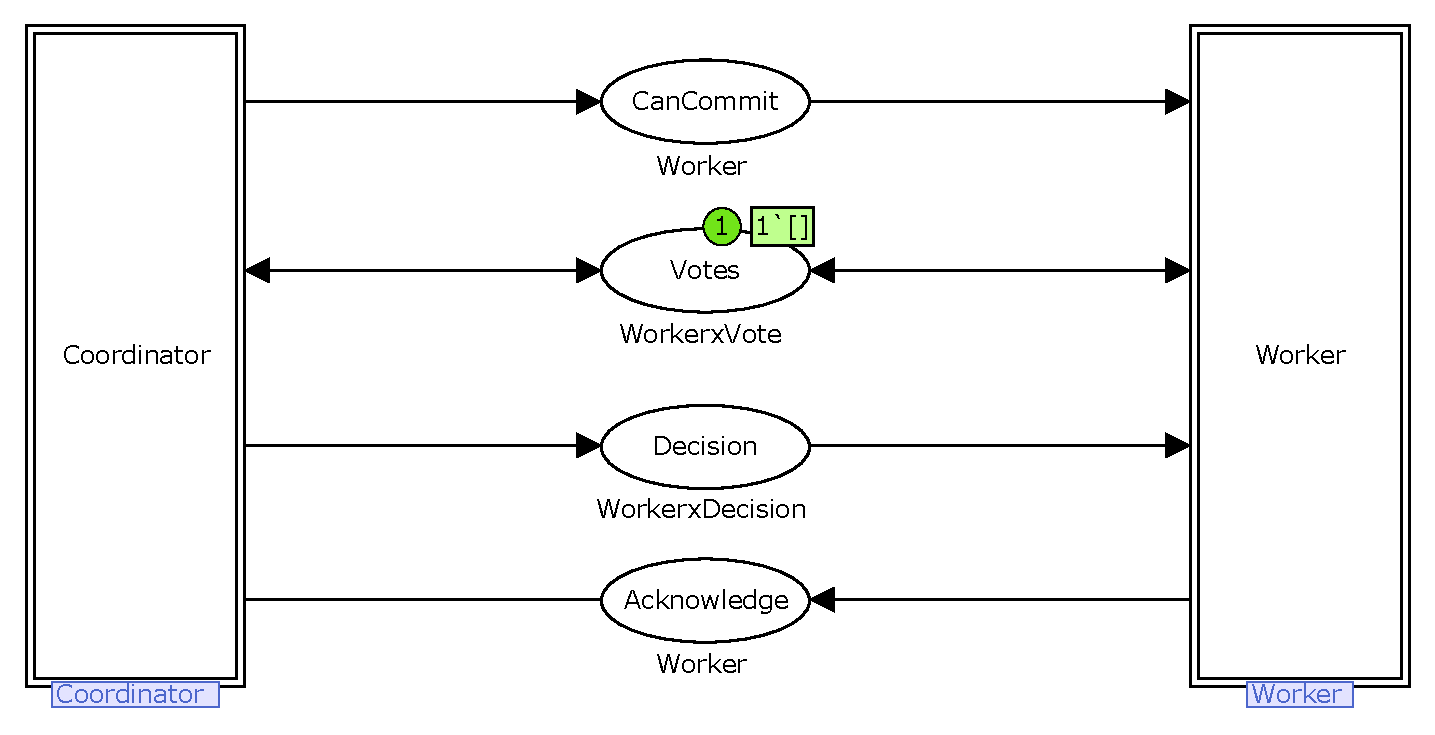
\includegraphics[width=15cm]{figures/Commit.eps}
\caption{The top-level Commit module of the CPN model.}
\end{figure*}

\begin{figure}[t]
\centering
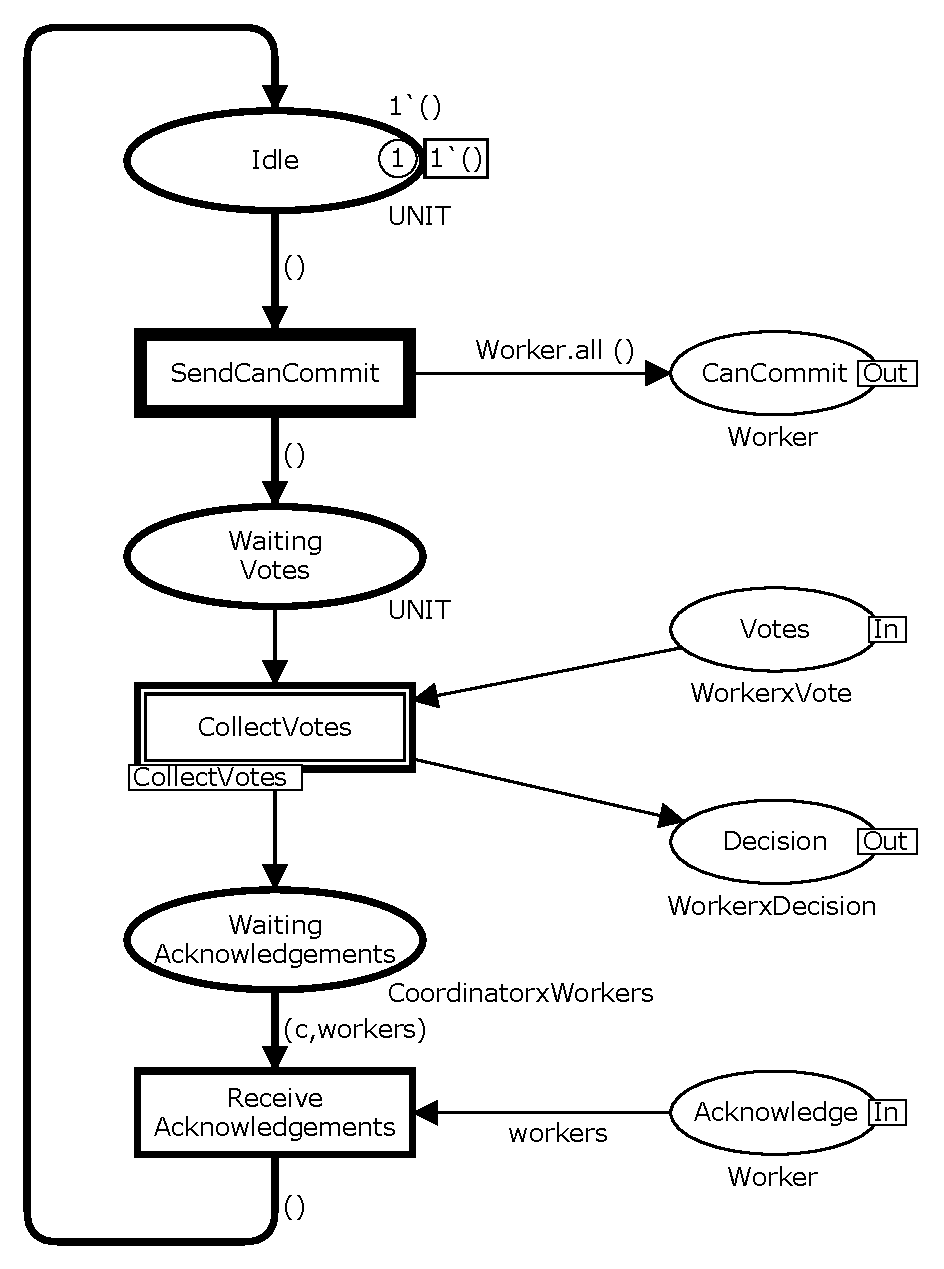
\includegraphics[width=\columnwidth]{figures/Coordinator.eps}
\caption{The Coordinator module.}
\end{figure}

\begin{figure}[t]
\centering
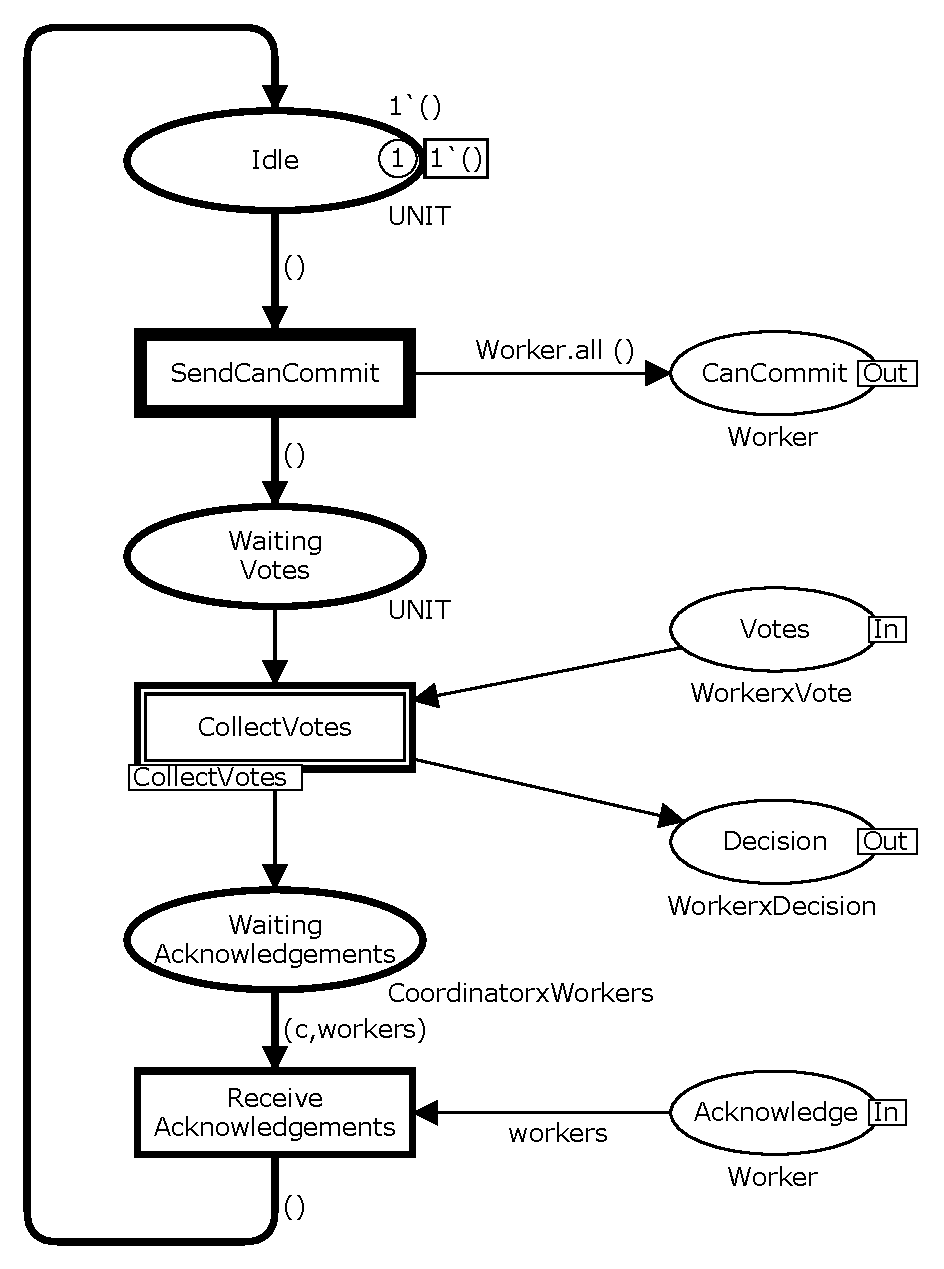
\includegraphics[width=\columnwidth]{figures/Coordinator.eps}
\caption{The CollectVotes module.}
\end{figure}

\begin{figure}[t]
\centering
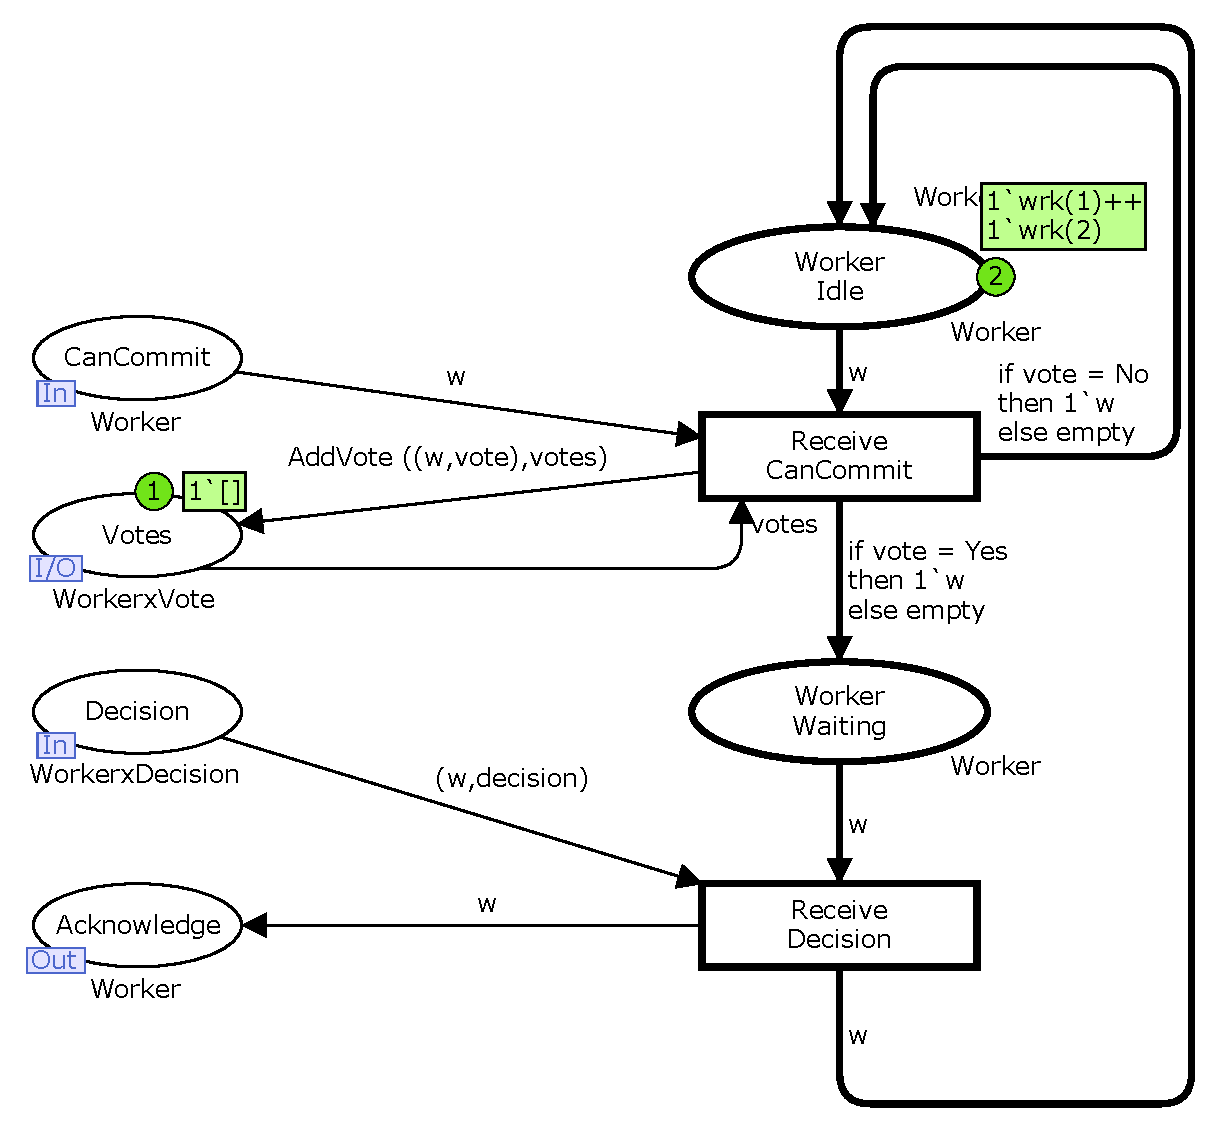
\includegraphics[width=\columnwidth]{figures/Worker.eps}
\caption{The Worker module.}
\end{figure}

\begin{figure}
\begin{verbatim}
colset INT = int;
var i : INT;

colset Coordinator = with c;
colset CoordinatorxInt = product Coordinator * INT;

colset Worker = index wrk with  1..2;
var w: Worker;

colset WorkerList = list Worker;
var workers : WorkerList;

colset CoordinatorxWorkers = product Coordinator * WorkerList;

colset Vote = with Yes | No;
var vote : Vote;

colset WorkerxVotes = product Worker * Vote;
colset WorkerxVote = list WorkerxVotes;
var votes : WorkerxVote;

colset Decision = with abort | commit;
var decision : Decision;

colset WorkerxDecision = product Worker * Decision;
\end{verbatim}
\caption{Colour sets and variable declarations.}
\end{figure}

\begin{figure}
\begin{verbatim}
val Workers = Worker.all();

fun AddVote ((w,vote),votes) = 
    sort_ms WorkerxVotes.lt ((w,vote)::votes);

fun YesWorkers votes = 
    List.map (fn (w,_) => w) 
      (List.filter (fn (w,Yes) => true 
                     | (w,No) => false) votes);

fun InformWorkers votes = 
    if (List.all (fn (_,Yes) => true 
                   | _ => false) votes)
                                            
    then List.map (fn w => (w,commit)) (YesWorkers votes)
    else List.map (fn w => (w,abort)) (YesWorkers votes);

fun All votes = List.length votes = List.length (Worker.all());
\end{verbatim}
\caption{Values and function definitions.}
\end{figure}
